\newpage
\section{Please be Rational}

Let's see if we can give yet another proof that the square root of two
is not rational. Consider the following isosceles right triangle:
\[
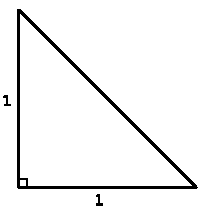
\includegraphics{../graphics/isorighttri.pdf}
\]
\begin{prob}
Using the most famous theorem of all, how long is the unmarked side?
\end{prob}

\begin{prob} 
Suppose that the unmarked side has a rational length. In that case how
could we express it?
\end{prob}

\begin{prob}
Explain why there would then be a \textit{smallest} isosceles right
triangle with integer sides. Considering the problem above, how long
would the sides be? Draw and label a picture.
\end{prob}

\newpage
\begin{prob}
Now fold your smallest isosceles right triangle with integer sides
along the dotted line like so:
\[
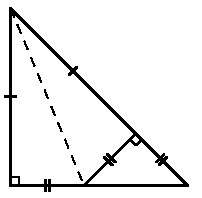
\includegraphics{../graphics/foldisorighttri.pdf}
\]
Explain why the segments we have marked above as ``equal'' are in fact
equal.
\end{prob}
\vspace{1in}

\begin{prob}
Explain how we have now found an isosceles right triangle with integer
sides that is now smaller than the smallest isosceles right triangle
with integer sides. Is this possible? What must we now conclude?
\end{prob}
